\chapter{Exponential- und Logartihmusfunktionen}

\subsection{Wiederholung: Exponentialfunktionen}

\begin{definition}
    Funktionen mit $f$ bzw. $g$ mit $$f(x) = a^x \text{ bzw. }g(x) = c \cdot a^x \text{  wobei } a, c \in \mathbb{R} \text{ mit } a > 0 \text{ und } a,c \neq 0$$ nennt man Exponentialfunktionen zur Basis $a$.
\end{definition}

\textit{Beispiele:}\footnote{Beachte beim Zeichnen, dass die Funktionen \textbf{nicht} die $x$-Achse schneiden. Am besten kurz davor mit dem Zeichnen aufhören.}

\begin{minipage}[b]{0.2\textwidth}
    (1): $\left(\frac{1}{2}\right)^x$ \\
    (2): $3 \cdot 2^x$ \\
    (3): $2 \cdot 2^x$ \\
    (4): $2^x$ \\
    (5): $-\left(\frac{1}{2}\right)^x$ \\
    (6): $-2 \cdot 2^x$ \\
    (7): $-2^x$
\end{minipage}
\begin{minipage}{0.8\textwidth}
    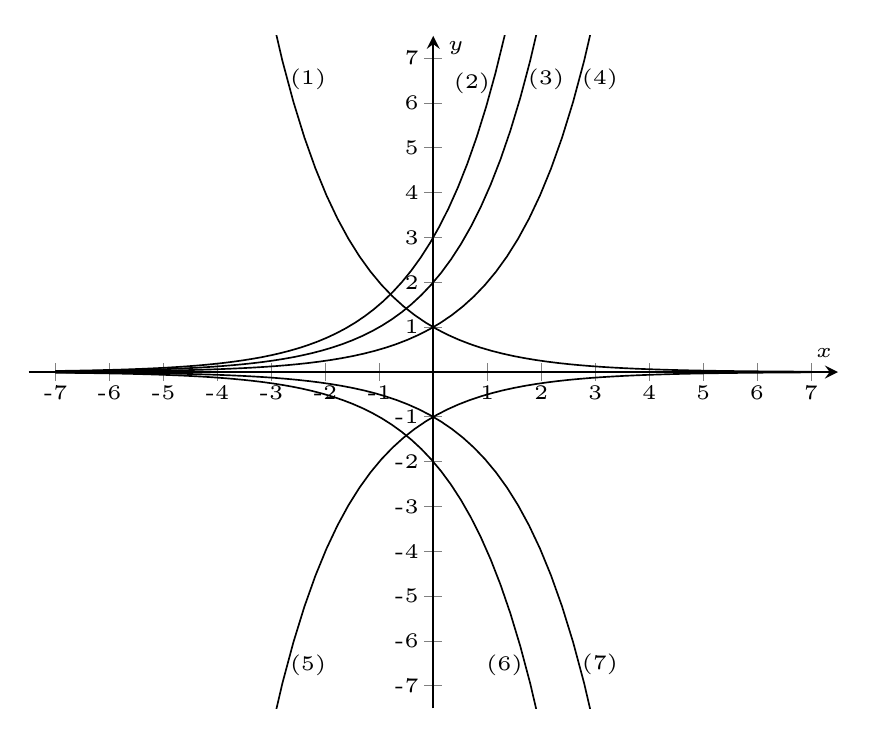
\begin{tikzpicture}[scale=1.5]
    \begin{axis}[clip=true, 
        xmin=-7.5, xmax=7.5, ymin=-7.5, ymax=7.5,
        axis lines = middle, 
        xlabel=$x$, ylabel=$y$,
        xlabel style = {font=\tiny,xshift=0.5ex},
        ylabel style = {font=\tiny,yshift=0.5ex},
        xtick={-7,-6,...,6,7}, xticklabels={-7,-6,...,6,7}, yticklabel style = {font=\tiny,xshift=0.5ex},
        xticklabel style = {font=\tiny,yshift=0.5ex},
        ytick={-7,-6,...,6,7}, yticklabels={-7,-6,...,6,7}]
    \addplot[samples=50, domain=-3:7]{(1/2)^x} node[xshift=5pt, pos=0.1]{\tiny(1)};
    \addplot[samples=50, domain=-7:1.5]{3*2^x} node[xshift=-5pt, pos=0.85]{\tiny(2)};
    \addplot[samples=50, domain=-7:1.98]{2*2^x} node[xshift=5pt, pos=0.9]{\tiny(3)};
    \addplot[samples=50, domain=-7:3]{2^x} node[xshift=5pt, pos=0.9]{\tiny(4)};
    \addplot[samples=50, domain=-3:7]{-(1/2)^x} node[xshift=5pt, pos=0.1]{\tiny(5)};
    \addplot[samples=50, domain=-7:1.98]{-2*2^x} node[xshift=-5pt, pos=0.9]{\tiny(6)};
    \addplot[samples=50, domain=-7:3]{-2^x} node[xshift=5pt, pos=0.9]{\tiny(7)};
    \end{axis}
    \end{tikzpicture}
\end{minipage} 

\textbf{Eigenschaften der Exponentailfunktionen zur Basis a}\\
Eigenschaften der Graphen $f$ mit $f(x) = a^x, a>0, a\neq1$:
\begin{outline}
    \1 sie verlaufen oberhalb der $x$-Achse, d. h. die Funktionswerte von $f$ sind alle positiv (>0) 
    \1 sie gehen durch den Punkt $P(0 \ | \ 1)$, denn es gilt $a^0 = 1$
    \1 sie sind für
    \2 $a>1$ streng monoton wachsend
    \2 $a<1$ streng monoton fallend
    \1 die $x$-Achse ist \textbf{waagrechte Asymptote}, d.h. die Werte von $f$ näheren sich der $x$-Achse, entweder für $x \to \infty$ oder $x \to -\infty$
\end{outline}
Die Graphen der Funktion $g$ mit $g(x) = c\cdot a^x$ gehen aus denen von $f$ mit $f(x)=a^x$ durch Streckung mit denm Faktor $c$ in $y$-Richtung hervor.

Falls $c<0$, erfolgt eine Spiegelung an der $x$-Achse.

Das große Anwendungsgebiet der Exponentialfunktionen ist die Beschreibung von Wachstumsvorgängen. Dabei werden auch Zerfallsvorgänge mit ihrer Hilfe beschrieben.

Die Basis $a$ im Funktionsterm der allgemeinen Exponentialfunktionen heißt auch Wachstumsfaktor.

\section{Die natürliche Exponentialfunktion und die Euler'sche Zahl e}

\begin{satz}
    Für die Funktion $f$ mit $f(x) = a^x$ gilt $f^\prime(x) = f^\prime(0) \cdot a^x$. Wenn $f^\prime(0) = 1$ ist, dann gilt $$f^\prime(x) = a^x \text{ ,also } f(x) = f^\prime(x)$$
\end{satz}

\begin{satz}
    Fie Funktion $f(x) = e^x$ ist diejenige Funktion, dür die gilt: $f(x) = f^\prime(x) = e^x$. Sie heißt natürliche Exponentialfunktion. $e$ ist die Euler'sche Zahl ($e \approx 2,718$).
\end{satz}

\ \\
\ \\

\begin{minipage}{0.5\textwidth}
    \textit{Beispiele:}
    \begin{equation*}
        \begin{gathered}
            f(x) = 2 + e^x \\
            f^\prime(x) = e^x\\
            \ \\
            f(x) = -5e^x \\
            f^\prime(x) = -5e^x \\
            \ \\
            f(x) = e^{5x} \\
            f^\prime(x) = 5 e^{5x} \\
            \ \\
            f(x) = e^{3x +2} \\
             f^\prime(x) = 3e^{3x + 2}
        \end{gathered}
    \end{equation*}
\end{minipage}
\begin{minipage}{0.5\textwidth}
    Graph der natürlichen Exponentialfunktion \\ $f(x) = e^x$
    
    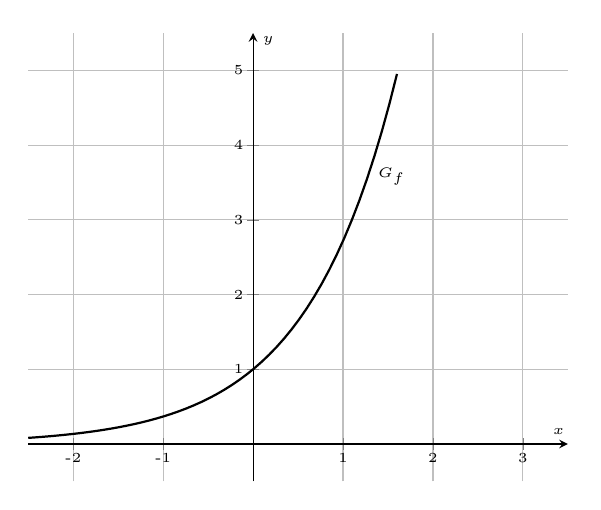
\begin{tikzpicture}[scale=1]
    \begin{axis}[clip=true, 
        xmin=-2.5, xmax=3.5, ymin=-0.5, ymax=5.5,
        axis lines = middle, 
        xlabel=$x$, ylabel=$y$,
        xlabel style = {font=\tiny,xshift=0.5ex},
        ylabel style = {font=\tiny,yshift=0.5ex},
        xtick={-7,-6,...,6,7}, xticklabels={-7,-6,...,6,7}, yticklabel style = {font=\tiny,xshift=0.5ex},
        xticklabel style = {font=\tiny,yshift=0.5ex},
        ytick={-7,-6,...,6,7}, yticklabels={-7,-6,...,6,7}, grid = major]
    \addplot[thick, samples=50, domain=-2.5:1.6]{(e^x} node[right, pos=0.8]{\tiny$G_f$};
    \end{axis}
    \end{tikzpicture}
\end{minipage}

\section{Exponentialgleichung und der natürliche Logarithmus}

\textit{Wiederholung:}

\begin{minipage}{0.5\textwidth}
    (1) $4^x = 12 \Rightarrow x = \log_{4}(12)$ \\
    (2) $a^x = y \Rightarrow x = \log_{a}(y)$
\end{minipage}
\begin{minipage}{0.5\textwidth}
    (3) $e^x = 12 \Rightarrow x = \log_{e}(12)$ \\
    (4) $e^x = y \Rightarrow x = \log_{e}(y)$ 
\end{minipage}

\begin{definition}
    $\log_{e}(y) =\ln{(y)}$\footnote{vor allem bei einfachen Ausdrücken auch manchmal ohne Klammern: $\ln{y}$} heißt \textbf{natürlicher Logarithmus} von $y$ und ist die Lösung der Gleichung $e^x = y$. \\Beachte: $y>0$, da $e^x >0$
\end{definition}
\noindent\rule{\textwidth}{1pt}

\textit{Beispiele:}

(1) $\ln{2} \approx 0,69$ (da $e^{0,69} \approx 2$) \\
(2) $\ln{0,25} \approx -1,39$ \\
(3) $\ln{(-3)}:$ nicht definiert

\textit{\textbf{Merke:}}

\begin{minipage}{0.5\textwidth}
    (1) $\ln{1} = 0$ (da $e^0 = 1$) \\
    (2) $\ln{e} = 1$ (da $e^1 = 1$) \\
    (3) $\ln{e^2} = 2$ (oder: $\ln{e^2} = 2 \cdot \ln{e} = 2$
\end{minipage}
\begin{minipage}{0.5\textwidth}
    (4) $\ln{e^x} = x$ \\
    (5) $\ln{\frac{1}{e}} = -1$ ($=\ln{e^{-1}})$ \\
    (6) $e^{\ln{e}} = x$
\end{minipage}


\subsection{Einschub: Ableitung der Exponentialfunktion}
Ges.: $f^\prime(x)$ für $f(x) = a^x$

Bsp.: $f(x) = 2^x = (e^{\ln{2}})^x = e^{\ln{2} \cdot x}$

\qquad \ $f^\prime(x) = \ln2 \cdot e^{\ln{2} \cdot x} = \ln{2} \cdot 2^x$

allgemein: 

$f(x) = a^x = e^{\ln{a} \cdot x}$\\
$f^\prime(x) = \ln{a} \cdot e^{\ln{a} \cdot x} = \ln{a} \cdot a^x$

\noindent\rule{\textwidth}{1pt}

\textit{Beispiele:}

\begin{minipage}[t]{0.5\textwidth}
    \begin{equation*}
        \begin{aligned}
            \text{(1.1) } && e^x &= 15 \\
            && x &= \ln{15} \approx 2,708 \\
            \ \\
            \text{(1.3) } && 3 \cdot e^{4y + 1} &= 16,2 \\
            && e^{4y + 1} &= 5,4 \\
            && 4y +1 &= \ln{5,4} \\
            && y &= \frac{1}{4}(\ln{(5,4)}-1) \approx 0,172 \\
            \ \\
            \text{(2.1) } && e^x &= e \\
            && x &= 1 \\
            \ \\
            \ \\
            \text{(2.3) } && 2 \cdot e^{7x -3} &= \sqrt{4e} \\
            && 2 \cdot e^{7x -3} &= 2\sqrt{e} \\
            && e^{7x -3} &= \sqrt{e} \\
            && 7x &= \frac{7}{2} \\
            && x &= \frac{1}{2}
        \end{aligned}
    \end{equation*}
\end{minipage}
\begin{minipage}[t]{0.5\textwidth}
    \begin{equation*}
        \begin{aligned}
            \text{(1.2) } && 4\cdot e^{-x} &= 10 \\
            && x &= - \ln{2,5} \approx -0,916 \\
            \ \\
            \text{(1.4) } && 3 + 2\cdot e^{3-4a} &= 9 \\
            && 4- 4a &= \ln{3} \\
            && a &= \frac{1}{4}(3 - \ln{3}) \approx0,475 \\
            \ \\
            \ \\
            \text{(2.2) } && e^{x -1} &= \sqrt{e} \\
            && x &= \frac{3}{2} \\
            \ \\
            \text{(2.4) } && e^{-4z} &= \frac{1}{e^2} \\
            && z &= \frac{1}{2}
        \end{aligned}
    \end{equation*}
\end{minipage}

\ \\
\ \\
\ \\

\subsection{Lösen von Exponentialgleichungen}

(1) Strategie: $e^x$ ausklammern
\begin{equation*}
    \begin{aligned}
        && e^{2x} - 3e^x & = 0 && \\
        && e^x(e^x -3) & = 0 && \\
        \ \\
        \text{S. v. Np.: } \text{ (1) } && e^x & \neq 0 \text{ für alle } x \in \mathbb{R} && \\
        \text{ (2) } && e^x - 3 & = 0 &&\\
        && x & = \ln{3} &&
    \end{aligned}
\end{equation*}

(2) Strategie: Multiplizieren mit $e^x$
\begin{equation*}
    \begin{aligned}
        e^x - 3e^{-x} & = 0 \\
        e^x - \frac{3}{e^x} & = 0 \qquad | \cdot e^x \\
        e^{2x} - 3 & = 0 \\
        x & = \frac{1}{2} \ln{3}
    \end{aligned}
\end{equation*}


(3) Strategie: Substitution $u = e^x$

{\centering $e^{2x} - 3e^x + 2 = 0$\par }

\begin{minipage}{0.5\textwidth}
    \begin{align*}
    \text{Substitution: } u & = e^x \\
    u^2 - 3u + 2 & = 0 \\
    \text{Mitternachtsformel:} & \\
    u_{1,2} & = \frac{3 \pm \sqrt{9 - 8}}{2} \\
     &= \frac{3 \pm 1}{2} \\
    \Rightarrow u_1 = 2 \quad u_2 & = 1 \\
\end{align*}
\end{minipage}
\begin{minipage}{0.5\textwidth}
    \begin{align*}
    \text{Resubstitution:} \\
    \text{(1) } e^x & = 2 \\
    x_1 & = \ln{2} \\
    \text{(2) } e^x & = 1 \\
    x_2 & = \ln{1} = 0
\end{align*}
\end{minipage}

(4)
\begin{align*}
    e^x - 2 e^{-x} +1 & = 0 \\
    e^x - \frac{2}{e^x} +1 & = 0  && | \cdot e^x\\
    e^{2x} -2 + e^x & = 0  && | \text{ Substitution: } u = e^x \\
    u^2 + u -2 & = 0 \\
\end{align*} 

(5)
\begin{align*}
    \left(e^x - \frac{1}{2}\right) \left(1 - e^x\right) = 0 \\
\end{align*} 
S. v. Np.:

\begin{minipage}[t]{0.5\textwidth}
    \begin{align*}
        \text{(1) }e^x - \frac{1}{2} & = 0 \\
        x & = \ln{\frac{1}{2}} = \ln{1} - \ln{2} \\
        x_1 & = - \ln{2}
    \end{align*}
\end{minipage}
\begin{minipage}[t]{0.5\textwidth}
    \begin{align*}
        \text{(2) }1 - e^x & = 0\\
        x_2 & = \ln{1} = 0
    \end{align*}
\end{minipage}

\section{Graphen von Exponentialfunktionen}
\subsection{Verhalten für $x \to \pm \infty$}
\textit{Beispiel:}

$f(x) = x^2e^{2x}$

Für $x \to \infty$ gilt: $f(x) \to \infty$ \\
Für $x \to - \infty$ gilt: $f(x) \to 0$

Der Graph von $f$ nähert sich für $x \to \infty$ der $x$-Achse, die Gerade $y = 0$ ist eine \textbf{waagrechte Asymptote} des Graphen von $f$ für $x \to \infty$.

\noindent\rule{\textwidth}{1pt}

\textit{Weitere Beispiele für Verhalten von $x \to \pm \infty$ bei Exponentialfunktionen:}

\begin{minipage}{0.43\textwidth}
    Für $x \to +\infty$ gilt \quad $e^x \to +\infty$ \\
    Für $x \to -\infty$ gilt \quad $e^x \to 0$ \\
    \ \\
    Für $x \to +\infty$ gilt \quad $e^{-x} \to 0$ \\
    Für $x \to -\infty$ gilt \quad $e^{-x} \to +\infty$ \\
    \ \\
    \textbf{Merke:} Für große Werte von $x$ \textbf{wächst} $e^x$ stets \textbf{\glqq schneller\grqq} als $x^n$\\
    \ \\
    Für $x \to +\infty$ gilt \quad $\frac{e^x}{x^n} \to +\infty$ \\
    Für $x \to -\infty$ gilt \quad $\frac{e^x}{x^n} \to 0$ \\
\end{minipage}
\begin{minipage}[t]{0.01\textwidth}
    \
\end{minipage}
\begin{minipage}{0.56\textwidth}
    Für $x \to +\infty$ gilt \quad $\frac{x^n}{e^x} \to 0$ \\
    Für $x \to -\infty$ gilt \quad $\frac{x^n}{e^x} \to +\infty$ (n gerade)\\
    $\land$\qquad \qquad \qquad \quad \ \ \qquad $\to -\infty$ (n ungerade) \\
    \ \\
    Für $x \to +\infty$ gilt \quad $x^n \cdot e^x \to +\infty$ \\
    Für $x \to -\infty$ gilt \quad $x^n \cdot e^x \to 0$ \\
    \ \\
    Für $x \to +\infty$ gilt \quad $e^x - x^n \to +\infty$ \\
    Für $x \to -\infty$ gilt \quad $e^x - x^n \to -\infty$ (n gerade) \\
    $\land$\qquad \qquad \qquad \qquad \quad \, \ \qquad $\to +\infty$ (n ungerade) \\
    \ \\
\end{minipage}

\subsection{Untersuchen auf Symmetrie}
\begin{satz}
    Ein Graph $f$ ist \textbf{achsensymmetrisch} zur $y$-Achse wenn $f(-x) = f(x)$ gilt. \\
    \phantom \qquad \ \ \ \ \ \, Ein Graph $f$ ist \textbf{punktsymmetrisch} zum Ursprung wenn $f(-x) = -f(x)$ gilt. 
\end{satz}

\textit{Beispiele:} \\
(1)
\begin{align*}
    f(x) & = 5xe^{-x^2} && \\
    f(-x) & = 5(-x)e^{-(-x^2)} = -5xe^{-x^2} = -f(x) &&
\end{align*}
$\rightarrow$ Der Graph von $f$ verläuft punktsymmetrisch zum Ursprung, da $f(-x) = -f(x)$

(2)
\begin{align*}
    f(x) & = e^{x^2}\left(e^{-2x} + e^{2x}\right) && \\
    f(-x) & = e^{x^2}\left(e^{2x} + e^{-2x}\right) &&
\end{align*}
$\rightarrow$ Der Graph von $f$ ist achsenysmmetrisch zur $y$-Achse, da $f(-x) = f(x)$

\section{Exponentailfunktionen mit Parameter}

\begin{definition}
    Enthält eine Funktion $f$ neben der unabhängigen Variablen $x$ noch einen \textbf{Parameter}, z. B. $t$, so gehört zu jedem $t$ eine Funktion $f_t$, die jedem $x$-Wert den Funktionswert $f_t(x)$ zuordnet. Die Funktionen $f_t$ bilden eine \textbf{Funktionenschar} von Funktionen.
\end{definition}
\textit{Beispiel:} \\
$f_t(x) = e^{2t - x} + x - 3t$\\
$f^\prime_t(x) = -e^{2t-x} + 1$\\
$f^{\prime\prime}_t(x) = e^{2t - x}$

Wir können Funktionsscharen wie Funktionen auf charakteristische Eigenschaften untersuchen, z. B. Symmetrie, Nullstellen, Extremstellen, Verhalten für $|x| \to \infty$, Asymptoten 

\textit{Beispiel:}\\
$f^\prime_t(x) = 0 \Longleftrightarrow 0 = -e^{2t - x} \Longleftrightarrow x = 2t$\\
$f^{\prime\prime}_t(x) = e^0 = 1 \Rightarrow \text{ Minimumstelle}$ \\
Also: $T_t( 2t \ | \ 1-t )$

Um ein Schaubild $K_f$ einer Funktion $f_t$ zu zeichnen, berechnen wir noch die fehlenden $y$-Werte der Punkte bzw. auch noch einen Schnittpunkt mit der $y$- Achse. 

\textit{Beispiel:}\\
$f_t(0) = e^{2t} -3t \Rightarrow S_y\left(0 \ | \ e^{2t} -3t \ \right)$
\begin{definition}
    \textbf{Ortskurve:} Ist nicht nur eine Funktion $f$, sondern eine Funktionenschar $f_t$ mit dem Parameter $t$ gegeben, sind häufig die Koordinaten bestimmter Punkte $P_t$ (z. B. Extrem- oder Wendepunkte) von $t$ abhängig. Durchläuft $t$ alle zugelassenen Werte, so bilden die Punkte $P_t$ eine Kurve. Diese Kurve heißt \textbf{Ortslinie}, \textbf{Ortskurve} oder \textbf{geometrischer Punkt} der Punkte $P_t$. \\
    Die zugehörigen Gleichung ergibt sich, indem wir $t$ aus den beiden Gleichungen $x = x(t)$ und $y = y(t)$ eliminieren.
\end{definition}
\textit{Beispiel:} \\
$T_t(2t \ | \ 1-t )$ \\
$x = 2t \Longleftrightarrow t = \frac{x}{2} \ (*)$\\
$(*) \text{ in } y = 1 - t: y = 1 - \frac{x}{2}$

Manche Funktionsscharen besitzen gemeinsame Punkte, d. h. es gibt Punkte, die auf allen zugehörigen Schaubildern liegen, wenn $t$ alle zugelassenen Werte durchläuft. Sie sind dann unabhängig von $t$. 

\textit{Beispiel:}\\
$f_a(x) = f_b(x) \qquad , a \neq b$\\
Die gesuchten Punkte sind unabhängig vom Parameter.

\noindent\rule{\textwidth}{1pt}

\textit{weiteres Beispiel:} \\
Gegeben ist die Funktionenschar $f_a$ mit $f_a(x) = e^x - a$ \ ($a \in \mathbb{R}$)\\
a) Geben sie $f_3(x)$, $f_{-2}(x)$ und $f_0(x)$ an.\\
b) Beschreiben Sie, wie sich eine Erhöhung von $a$ auf die Lage der Graphen auswirkt.\\
c) Bestimmen Sie die Ableitung von $f_a$

a) $f_3(x) = e^x -3$, $f_{-2}(x) = e^x +2$, $f_0(x) = e^x$ \\
b) Eine Erhöhung von $a$ bewirkt eine Verschiebung des Graphen nach unten. \\
c) $f^\prime_a(x) = e^x$
\ \\
\ \\
\ \\
\ \\
\ \\
\ \\
\ \\
\ \\
\section{Die Umkehrfunktion}

\begin{definition}
    Eine Funktion $f$ mit der Definitonsmenge $D_f$ und Wertemenge $W_f$ heißt \textbf{umkehrbar}, falls es zu jedem $y \in W_f$ genau ein $x \in D_f$ mit $f(x) = y$ gibt. \\
    Bei einer umkehrbaren Funktion $f$ heißt die Funktion $\bar{f}$ mit $\bar{f}(y) = x$ (wobei $f(x) = y$ ist) die \textbf{Umkehrfunktion} von $f$. Sie hat die Defintionsmenge $D_{\bar{f}} = W_f$ und die Wertemenge $W_{\bar{f}} = D_f$.
    $$\text{Es gilt } \bar{f}(f(x)) = x \text{ für alle } x \in D_f \text{ und } f(\bar{f}(x)) = x \text{ für alle } x \in D_{\bar{f}} = W_f$$
\end{definition}

\begin{minipage}{0.35\textwidth}
    \textit{Beispiel} \\
    $f(x) = x^2$ \quad mit $D_f = \mathbb{R}^+_0$ \\
    
    $\Rightarrow$ Der Graph von $\bar{f}$ entsteht aus dem Graphen von $f$ durch Spiegelung an der 1. Winkelhalbierenden.
    \begin{align*}
        \Rightarrow f(x) & = x^2 \\
        y & = x ^2 \\
        x & = \sqrt{y} \text{ oder } x = -\sqrt{y}
    \end{align*}
    Da $x \in \mathbb{R}^+_0$, trifft der 1. Fall zu \\
    Also: $y= \sqrt{x}$ \\
    $\bar{f}(x) = \sqrt{x}$
    
\end{minipage}
\begin{minipage}{0.65\textwidth}
    \begin{tikzpicture}[scale=1.5]
        \begin{axis}[clip=false, 
            xmin=-2.5, xmax=4.5, ymin=-1.5, ymax=4.5,
            axis lines = middle, 
            xlabel=$x$, ylabel=$y$,
            xlabel style = {font=\tiny,xshift=0.5ex},
            ylabel style = {font=\tiny,yshift=0.5ex},
            xtick={-2,-1,...,3,4}, xticklabels={-2,-1,...,3,4}, yticklabel style = {font=\tiny,xshift=0.5ex},
            xticklabel style = {font=\tiny,yshift=0.5ex},
            ytick={-1,0,...,3,4}, yticklabels={-1,0,...,3,4}, grid = major]
        \draw[] (0,0) -- (4,4) node[pos=0.98, above]{\tiny1. Winkelhalbierende};
        \draw[dashed] (1.732,3) -- (3,1.732);
        \draw[]  (1.732,3) node[cross] {} node[above right] {\tiny$P(a | b)$};
        \draw[]  (3,1.732) node[cross] {} node[below right] {\tiny$Q(b | a)$};
        \coordinate (A) at (2.4, 2.4);
        \coordinate (B) at (2.35, 2.35);
        \coordinate (C) at (2.38, 2.325);
        \draw pic [draw,angle radius=0.2cm] {angle = C--B--A};
        \node[] at (2.475,2.355) {\tiny$\cdot$};
        \addplot[blue, domain=0:2, samples=50]  {x^2} node[left]{\tiny$G_f$};
        \addplot[red, domain=0:4, samples=100]  {sqrt(x)} node[above]{\tiny$G_{\bar{f}}$};
        \end{axis}
    \end{tikzpicture}
\end{minipage}

\textbf{Bestimmung des Funktionsterms der Umkehrfunktion}

Gegeben ist eine Funktion $f$, die auf der Definitionsmenge $D_f$ umkehrbar ist
\begin{enumerate}
    \item $y = f(x)$ setzen.
    \item Gleichung nach $x$ auflösen.
    \item $x$ und $y$ vertauschen. 
    \item $y$ durch $\bar{f}$ ersetzen.
\end{enumerate}

\textbf{Überprüfung auf Umkehrbarkeit}
\begin{satz}
    Jede streng monotone Funktion ist umkehrbar. Insbesondere ist jede in einem Intervall $I$ differenzierbare Funktion $f$ mit $f^\prime(x) > 0$ bzw. $f^\prime(x) < 0$ für alle $x \in I$ umkehrbar. \footnote{Die strenge Monotonie ist auch erfüllt, wenn für ein $x \in D_f$ (bzw. $x \in I$), das am Rand von $D_f$ (bzw. $I$) liegt, entweder $f^\prime(x) = 0$ gilt oder $f^\prime$ nicht definiert ist.}
\end{satz}

\textit{Beispiel}

$f(x) = \sqrt{4x-2} + 1$\\
$D_f = [0,5 ; \infty[ \ \ \land \ \ W_f = [1 ; \infty[$\\

Überprüfung auf Umkehrbarkeit:
\begin{align*}
    f(x) & = \sqrt{4x-2} + 1 \text{ mit } D_f = [0,5 ; \infty[ && \\
    f^\prime(x) & = \frac{2}{\sqrt{4x - 2}} > 0 \text{ für } x > 0,5 && 
\end{align*}
$\Rightarrow$ Somit ist $f$ auf $D_f$ streng monoton wachsend und damit umkehrbar.

Bestimmen der Umkehrfunktion:
\begin{align*}
    y & = \sqrt{4x-2} + 1 &&\\
    y -1 & = \sqrt{4x-2} &&\\
    (y-1)^2 & = 4x - 2 &&\\
    (y-1)^2 + 2 & = 4x &&\\
    x & = \frac{1}{4} ((y-1)^2 + 2) &&
\end{align*}
Also: $\bar{f}(x) = \frac{1}{4}(y-1)^2 + \frac{1}{2}$ mit $D_{\bar{f}}= W_f$ und $W_{\bar{f}}= D_f$

\section{Die Logarithmusfunktion und ihre Ableitung}

\begin{minipage}{0.35\textwidth}
    Geg.: $f(x) = e^x$\\
    Ges.: Umkehrfunktion $\bar{f}$
    \begin{align*}
        y & = e^x && \\
        \ln{(y)} & = x && \\
        y & = \ln{(x)} &&
    \end{align*}
    Also: $\bar{f}(x) = \ln{(x)}$
\end{minipage}
\begin{minipage}{0.65\textwidth}
    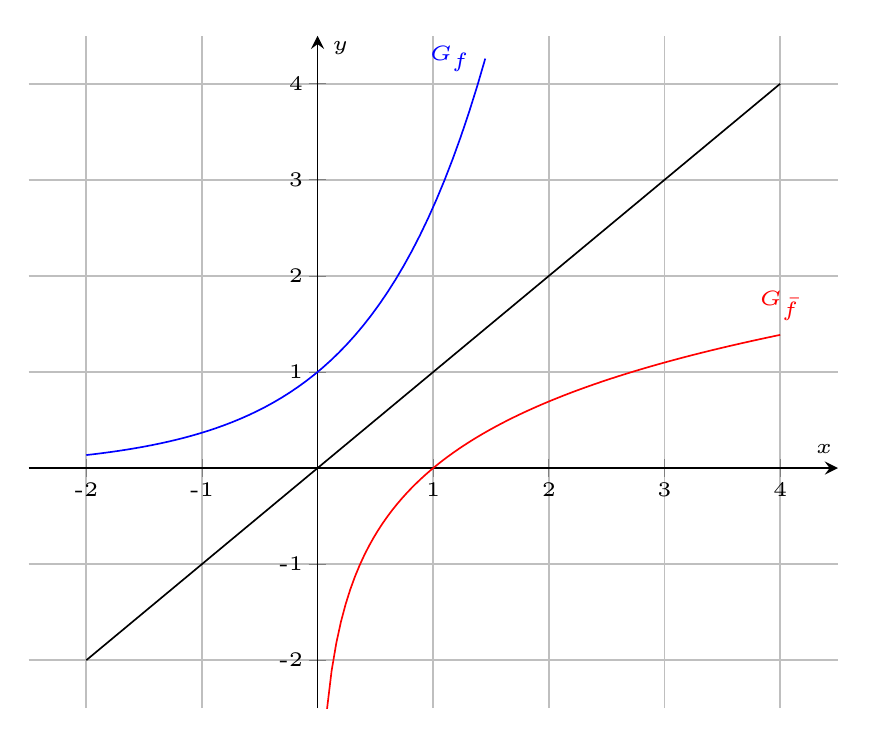
\begin{tikzpicture}[scale=1.5]
        \begin{axis}[clip=true, 
            xmin=-2.5, xmax=4.5, ymin=-2.5, ymax=4.5,
            axis lines = middle, 
            xlabel=$x$, ylabel=$y$,
            xlabel style = {font=\tiny,xshift=0.5ex},
            ylabel style = {font=\tiny,yshift=0.5ex},
            xtick={-2,-1,...,3,4}, xticklabels={-2,-1,...,3,4}, yticklabel style = {font=\tiny,xshift=0.5ex},
            xticklabel style = {font=\tiny,yshift=0.5ex},
            ytick={-2,-1,...,3,4}, yticklabels={-2,-1,...,3,4}, grid = major]
        \addplot[domain=-2:4]{x};
        \addplot[blue, domain=-2:1.45, samples=50]  {e^x} node[left]{\tiny$G_f$};
        \addplot[red, domain=0:4, samples=100]  {ln(x)} node[above]{\tiny$G_{\bar{f}}$};
        \end{axis}
    \end{tikzpicture}
\end{minipage}
\begin{definition}
    Die \textbf{natürliche Logarithmusfunktion} mit $\bar{f}$ mit $\bar{f}(x) = \ln{(x)}$ ist die Umkehrfunktion der natürlichen Exponentialfunktion $f$ mit $f(x) = e^x$. Sie hat die maximale Definitionsmenge $D_{\bar{f}} = ]0;\infty[$ und ihre Wertemenge $W_{\bar{f}} = \mathbb{R}$.
\end{definition}

\textbf{Ableitung der natürlichen Logarithmusfunktion}\\
mit $f(\bar{f}(x)) = x$:
\begin{align*}
    x  & = e^{\bar{f}(x)} && \\
    (x)^\prime & = \left(e^{\bar{f}(x)}\right)^\prime && \\
    1 & = \bar{f}^\prime(x) \cdot e^{\bar{f}(x)} && \\
    1 & = \bar{f}^\prime(x) \cdot x && \\
    \bar{f}^\prime(x) & = \frac{1}{x} &&
\end{align*}

\subsection{$\ln$ Gesetze}
\begin{enumerate}
    \item $\ln{(\frac{1}{x})} = \ln{(1)} - \ln{(x)}$
    \item $\ln{(2x)} = \ln{(2)} + \ln{(x)}$
    \item $\ln{(a^x)} = x \cdot \ln{(a)}$
\end{enumerate}
\noindent\rule{\textwidth}{1pt}
\textit{Beispiel}

$f(x) = 4 \cdot e^{3x-2} + 1$ \\
$D_f = \mathbb{R} \ , \ W_f = \ ] 1 ; \infty [$ \\
$f^\prime(x) = 12 \cdot e^{3x-2} > 0$ Also ist $f$ streng monoton wachsend auf ganz $\mathbb{R}$. Somit ist $f$ umkehrbar.
\begin{align*}
    y & = 4 \cdot e^{3x-2} + 1 && \\
    \frac{y - 1}{4} & = e^{3x-2} && \\
    \ln{\left(\frac{y - 1}{4}\right)} & = 3x-2 && \\
    x & = \frac{1}{3}\left(\ln{\left(\frac{y - 1}{4}\right)} + 2\right) && \\
    y & = \frac{1}{3}\left(\ln{\left(\frac{y - 1}{4}\right)} + 2\right) && \\
    \bar{f}(x) & = \frac{1}{3}\left(\ln{\left(\frac{y - 1}{4}\right)} + 2\right) \qquad D_{\bar{f}} = \ ] 1 ; \infty [ \ \ W_{\bar{f}} = \mathbb{R} &&
\end{align*}

\section{Anwendungen von Exponentialfunktionen}
\subsection{Exponentielle Wachstums- und Zerfallsprozesse}
\begin{definition}
    Exponentielle \textbf{Wachstums- und Zerfallsprozesse} können durch Funktionen $f$ mit $$f(t) = c \cdot a^t \text{ bzw. } f(t) = c \cdot e^{k \cdot t} \text{ mit } k = \ln{(a)} \text{ und } a > 0$$ beschrieben werden. Dabei ist $c \in \mathbb{R}$ der \textbf{Anfangsbestand} $f(0)$ zum Zeitpunkt $t = 0, f(t)$ der Bestand zum Zeitpunkt $t$ und $a$ der \textbf{Wachstumsfaktor}.
    
    Für $0 < a <1$ ist $f$ eine Zerfallsfunktion (negatives Wachstum).\\
    Für $a > 1$ ist $f$ eine Wachstumsfunktion (positives Wachstum). 

    Für $k > 0$ heißt $k$ \textbf{Wachstumskonstante} und $f$ \textbf{Wachstumsfunktion}. \\
    Für $k < 0$ heißt $k$ \textbf{Zerfallskonstante} und $f$ \textbf{Zerfallsfunktion}.
\end{definition}
\noindent\rule{\textwidth}{1pt}
\textit{Beispiel:} Eine Bakterienkultur nimmt mit der Wachstumskonstante $k = 0,03\frac{1}{\text{min}}$ zu. \\
Nach 100 min wurden 800 Bakterien gezählt.\\
a) Wie groß war der Anfangsbestand?\\
b) Wie viele Bakterien werden nach 200 min vorhanden sein?

a) 
\begin{align*}
    f(t) & = c \cdot e^{0,03t}; f(100) = c \cdot e^{0,03 \cdot 100} = c \cdot e^3 && \\
    800 & = c \cdot e^3 \Rightarrow c = \frac{800}{e^3} \approx 39,82 &&
\end{align*}
A.: Der Anfangsbestand betrug ca. 40.

b) \begin{align*}
    f(200) & = 40 \cdot e^{0,03 \cdot 200} = 40 \cdot e^6 \approx 16 137,15 &&
\end{align*}
A.: Nach 200 min werden etwa 16 137 Bakterien vorhanden sein. 
\subsection{Zusammenhang zwischen $p$ und $k$}
Mit der Wachstums- bzw. Zerfallskonstante $k$ verbinden wir keine direkte anschauliche Vorstellung. Meist wird deshalb das Wachstum durch die prozentuale Zunahme $p$ pro Zeitschritt angegeben. \\

Es gilt für die Wachstumskonstante $k$ und die prozentuale Zunahme $p$ pro Zeitschritt: $$\text{Aus: } f(t+1) = a \cdot f(t) = f(t) + \frac{p}{100} \cdot f(t) = \left(1 + \frac{p}{100}\right) \cdot f(t) \text{ folgt } a = \left(1 + \frac{p}{100}\right)$$
Mit $k = \ln{(a)}$ ergibt sich $k = \ln{\left(1 + \frac{p}{100}\right)}$. Nach $p$ auflösen ergibt sich: $p = 100 \cdot \left(e^k - 1\right)$. \\

Analog gilt für die Zerkallskonstante $k$ und die prozentuale Abnahme pro Zeitschritt: $$\text{Aus: } f(t+1) = a \cdot f(t) = f(t) - \frac{p}{100} \cdot f(t) = \left(1 - \frac{p}{100}\right) \cdot f(t) \text{ folgt } a = \left(1 - \frac{p}{100}\right)$$
Mit $k = \ln{(a)}$ ergibt sich $k = \ln{\left(1 - \frac{p}{100}\right)}$. Nach $p$ auflösen ergibt sich: $p = 100 \cdot \left(1 - e^k\right)$.
\subsection{Berechnung der Halbwertzeit $T_H$ bzw. der Verdopplungszeit $T_V$} 
\begin{minipage}[t]{0.49\textwidth}
    Eine für den Zerfallsprozess charakteristische Größe ist die Halbwertszeit, d. h. die Zeit, in der sich der Bestand jeweils halbiert.\\

    Die Halbwertszeit $T_H$ eines Zerfalls berechnen wir folgendermaßen:

    \begin{align*}
        f(t + T_H) & = \frac{1}{2} f(t) \text{ mit } f(t) = c \cdot e^{k \cdot t} && \\
        c \cdot e^{k \cdot (t + T_H)} & = \frac{1}{2} c \cdot e^{k \cdot t} && \\
        c \cdot e^{k \cdot t} \cdot e^{k \cdot T_H} & = \frac{1}{2} c \cdot e^{k \cdot t} && \\
        e^{k \cdot T_H} & = \frac{1}{2} && \\
        k \cdot T_H & = \ln{\left(\frac{1}{2}\right)} && 
    \end{align*}
    Somit ergibt sich für die Halbwertszeit:
    \begin{align*}
        T_H & = \frac{\ln{\left(\frac{1}{2}\right)}}{k} \text{ oder } && \\
        T_H & = -\frac{\ln{(2)}}{k}
    \end{align*}
\end{minipage}
\begin{minipage}{0.02\textwidth}
    \
\end{minipage}
\begin{minipage}[t]{0.49\textwidth}
    Analog gilt für einen Wachstumsprozess und die Verdoppelungszeit $T_V$: \\
    \ \\
    \ \\
    \ \\
    \ \\
    \begin{align*}
        f(t + T_V) & = 2 f(t) \text{ mit } f(t) = c \cdot e^{k \cdot t} && \\
        c \cdot e^{k \cdot (t + T_V)} & = 2 c \cdot e^{k \cdot t} && \\
        c \cdot e^{k \cdot t} \cdot e^{k \cdot T_V} & = 2 c \cdot e^{k \cdot t} && \\
        e^{k \cdot T_V} & = 2 && \\
        k \cdot T_V & = \ln{(2)} && 
    \end{align*}
    \ \\
    \vspace{1.5pt}
    
    Somit ergibt sich für die Verdoppelungszeit:
    \begin{align*}
        T_V & = \frac{\ln{(2)}}{k}&& \\
    \end{align*}
\end{minipage}